\documentclass[twocolumn]{amsart}
\usepackage[top=0.5in, left=0.45in, right=0.45in, bottom=0.5in]{geometry}

\usepackage{url}
% \usepackage{code}
% \usepackage{cite}
\usepackage{amsmath}
\usepackage{amssymb}
\usepackage{graphicx}
\usepackage{chessboard}

% \usepackage{chessfs}
\usepackage{adjustbox}

% Define black versions of pieces for inline use. Gross, but it works.
\newcommand{\Pawn}[1][1.3ex]{%
\adjustbox{Trim=4.3pt 2.6pt 4.3pt 0pt,width=#1,margin=0.2ex 0ex 0.2ex 0ex}{\BlackPawnOnWhite}%
}%
\newcommand{\Rook}[1][1.58ex]{%
\adjustbox{Trim=3.2pt 2.2pt 3.2pt 0pt,width=#1,raise=0ex,margin=0.1ex 0ex 0.1ex 0ex}{\BlackRookOnWhite}%
}%
\newcommand{\Knight}[1][1.85ex]{%
\adjustbox{Trim=2.3pt 2.35pt 2.5pt 0pt,width=#1,raise=-0.03ex,margin=0.14ex 0ex 0.14ex 0ex}{\BlackKnightOnWhite}%
}%
\newcommand{\Bishop}[1][1.79ex]{%
\adjustbox{Trim=2.3pt 2pt 2.3pt 0pt,width=#1,raise=-0.12ex,margin=0.1ex 0ex 0.1ex 0ex}{\BlackBishopOnWhite}%
}%
\newcommand{\Queen}[1][2.05ex]{%
\adjustbox{Trim=1.2pt 2.2pt 1.2pt 0pt,width=#1,raise=-0.08ex,margin=0.1ex 0ex 0.1ex 0ex}{\BlackQueenOnWhite}%
}%
\newcommand{\King}[1][1.95ex]{%
\adjustbox{Trim=2pt 2pt 2pt 0pt,width=#1,raise=-0.06ex,margin=0.13ex 0ex 0.13ex 0ex}{\BlackKingOnWhite}%
}%

\interfootnotelinepenalty=0

% lets me explicitly set a. or 1. etc. as enum label
\usepackage{enumitem}

\pagestyle{empty}

\usepackage{ulem}
% go back to italics for emphasis, though
\normalem

\usepackage{natbib}

\setlength{\footnotesep}{2em}

% \newcommand\comment[1]{}
\newcommand\sfrac[2]{\!{}\,^{#1}\!/{}\!_{#2}}

\begin{document} 

\title{Color- and piece-blind chess}
\author{Dr.~Tom~Murphy~VII~Ph.D.}\thanks{
Copyright \copyright\ 2019 the Regents of the Wikiplia Foundation.
Appears in The Journal Of LaTeX Class Files with the insufficient
material of the Association for Computational Heresy; {\em IEEEEEE!}
press, Verlag-Verlag volume no.~0x40-2A. 1 tempo}

\setchessboard{showmover=false}

\newcommand\checkmate{\hspace{-.05em}\raisebox{.4ex}{\tiny\bf ++}}

\renewcommand\th{\ensuremath{{}^{\textrm{th}}}}
\newcommand\st{\ensuremath{{}^{\textrm{st}}}}
\newcommand\rd{\ensuremath{{}^{\textrm{rd}}}}
\newcommand\nd{\ensuremath{{}^{\textrm{nd}}}}
\newcommand\at{\ensuremath{\scriptstyle @}}

\date{1 April 2019}

\maketitle \thispagestyle{empty}

% \begin{abstract}
% CHESSMATE.
% \end{abstract}

\section*{Impressing humans}

What better way for humans to impress each other with their brains,
especially in movies, than to play chess---and to shout dramatically
CHECKMATE! upon surprise-checkmating their opponent? Well, one way is
to play chess while disadvantaged somehow, for example, by punching
each other in the face repeatedly during the game to impair brain
function (see Chess Boxing~\cite{chessboxing}). Another common
distraction is to play a multitude of games against many opponents at
the same time, in a so-called ``simultaneous exhibition.'' The idea is
that this is more challenging because of the need to maintain mental
state for so many games at once, whereas your opponents only need to
maintain state for one game. In truth, simultaneous exhibitions easily
fall to a ``man-in-the-middle attack.'' If the purported genius simply
creates a bipartite matching of the games played with the white pieces
and the games played with black, he can mechanically forward moves
between these pairs of boards. This requires only constant state (see
next section) per pair of games, and guarantees an even score for the
exhibition. So that's not very impressive.

Another disadvantage that humans sometimes use to impress each other
is a blindfold; they only hear the opponent announce the moves and
must keep the position on the board in their mind's eye, both for
the sake of remembering it and while exploring potential moves.
% This is effective, since although the .
Disadvantages can be combined, such as in the final scene of the 1988
documentary {\it Bloodsport} where Jean Claude van Damme is blinded by
an illicit foreign substance during the final martial art
battle.\footnote{JCVD does not play chess on camera, but it is implied
  that he is also holding a simultaneous exhibition between rounds in
  a different room of the underground Hong Kong illegal karate
  complex.}

\section{Impressing computers}

In contrast, it is much more difficult to impress computers or impress
people with computers. For example, it is well known that computers
function {\em better} when struck, so chess boxing becomes trivial.
Playing multiple games simutaneously is an easy extension of playing a
single game, and when it comes to computers playing chess, largely,
the jig is up; it is now easy for chess programs, running on consumer
hardware, to defeat the strongest human players. Blindfold chess is
the natural interface for a chess computer; it is actually {\em much
  more difficult} to have the computer interpret the opponent's move
by visually studying a physical board!

Computers can still impress us and each other with computational chess
feats other than playing. For example, computers are largely concerned
with filling up their memories with efficiently encoded data.

compactly storing a position. constant state

I think a version I liked was 64 bits (this gives the positions of all
pieces), followed by 32 records giving the piece values (there are 6:
pawn, knight, bishop, rook, queen, king) and colors. To pick between
the 12 possibilities we need 4 bits, and there is some slack here of
course. anyway, that's 64 + 32*4 = 192 bits, plus 15 bits for other
state. Note we could use the c_rook trick to save 4 bits for castling
rights (14 possibilities), not to mention a en_passantable pawn (15)
and a king whose turn it is (even 16). Clear slack here, but that
would leave only the 50-move rule at 7 bits, for a total of 199.
Wikipedia says the huffman approach is ``maximum of 204 bits, and
often much less.'' but the article also contains many bugs, like
the misconception that there can only be four rooks. 



% 
% % make -j eval-unblinder.exe && ./eval-unblinder.exe net.val
% .!Evaluating model net.val...
% Loaded 50000 positions in 122.59s
% Loaded model in 0.10s
% Ran eval in 2.04s
% Reading [net.val]
% net.val: 4 layers.
% net.val: num nodes: 64 1024 12288 567 837
% net.val: indices per node/fns: 49 LEAKY_RELU 36 LEAKY_RELU 127 LEAKY_RELU 78 LEAKY_RELU
% Read from net.val.
% Invert index:
% Check it:
% ModelInfo [339885 rounds, 223224128 examples]
% Over 50000 positions:
%   9584 exactly correct (19.17%)
%   161166 piece mistakes (3.22/pos)
%   1630 castling mistakes (0.03/pos)
%   19014 move mistakes (0.38/pos)
%   181810 total mistakes (3.64/pos)
% 
% % $ make -j eval-unblinder.exe && ./eval-unblinder.exe net-before-vacuum.val
% make: 'eval-unblinder.exe' is up to date.
% Evaluating model net-before-vacuum.val...
% Loaded 50000 positions in 118.80s
% Loaded model in 3.99s
% Ran eval in 332.10s
% Reading [net-before-vacuum.val]
% net-before-vacuum.val: 4 layers.
% net-before-vacuum.val: num nodes: 64 1024 12288 567 837
% net-before-vacuum.val: indices per node/fns: 64 LEAKY_RELU 1024 LEAKY_RELU 12288 LEAKY_RELU 567 LEAKY_RELU
% Read from net-before-vacuum.val.
% Invert index:
% Check it:
% ModelInfo [146999 rounds, 9407936 examples]
% Over 50000 positions:
%   10601 exactly correct (21.20%)
%   156052 piece mistakes (3.12/pos)
%   1542 castling mistakes (0.03/pos)
%   18818 move mistakes (0.38/pos)
%   176412 total mistakes (3.53/pos)
% 
% 
% 
% without concurrent processes:
% net.val: 1.61s  (something like 1035/sec/core)
% net-before-vacuum: 229.85s (something like 7/sec/core)
% 
% 
% single_kings net.val:
% Over 50000 positions:
%   9642 exactly correct (19.28%)
%   162804 piece mistakes (3.26/pos)
%   1633 castling mistakes (0.03/pos)
%   19014 move mistakes (0.38/pos)
%   183451 total mistakes (3.67/pos)
% 
% It's actually kind of heartening that it performs worse with this approach,
% though we are more likely to get the whole board correct.
% 
% (cite #kingme)
% 

% all bits set to 1 (with single_kings)
% (without single_kings, only difference is that the bottom right becomes a
% rook; no white queen)
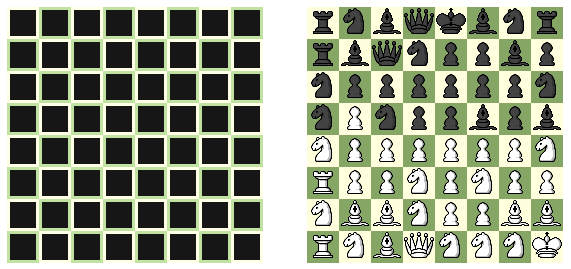
\includegraphics{blind-allon}

\bibliography{chess}{}
\bibliographystyle{plain}

\end{document}
